\mode*

\begin{frame}
\frametitle{Online Resources}

\begin{center}
\pdftooltip{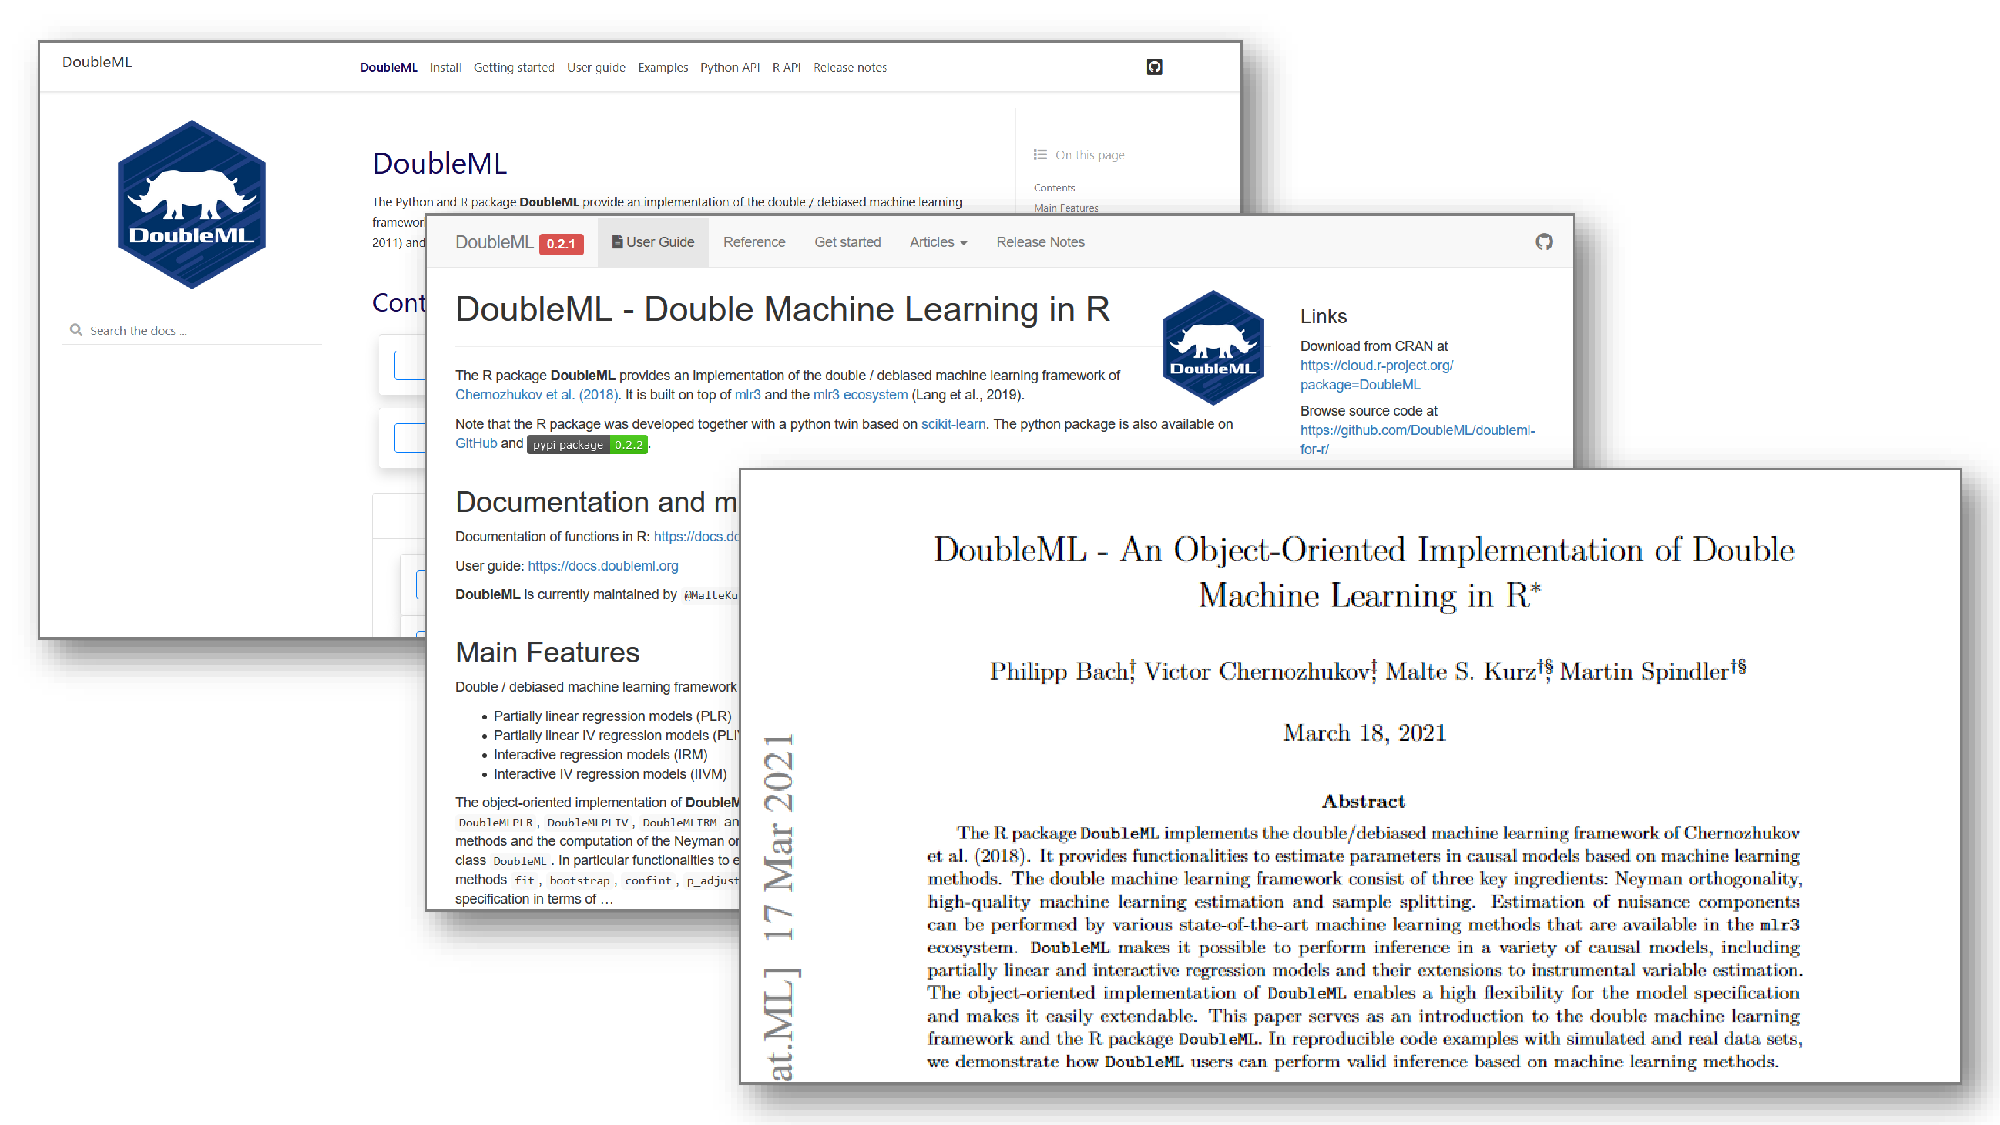
\includegraphics[width=0.8\textwidth]{pictures_and_logos/comingsoon_v3.pdf}}{An arrangement of three screenshots. The first screenshot on the left is a preview on the package website and user guide at https://docs.doubleml.org. The second screenshot which is in the middle is a preview on the documentation website of the R package available at https://docs.doubleml.org/r/stable/. The third screenshot (on the right) is a preview on the package vignette that is available at arxiv.}
\end{center}

\begin{itemize}
\item Documentation and User Guide available at
\begin{center}
\textbf{\url{https://docs.doubleml.org}}
\end{center}
\item Package vignette available via \href{https://arxiv.org/abs/2103.09603}{\textbf{arXiv:2103.09603}}
%\href{https://cran.r-project.org/web/packages/DoubleML/index.html}{\textbf{CRAN}} or
\end{itemize}
\end{frame}


\begin{frame}
\frametitle{Thank you, UseR!}

\begin{center}
\begin{large}
\textbf{Thank you very much for your attention!}
\end{large}
\end{center}
\vspace{20pt}
\begin{center}
\href{mailto:philipp.bach@uni-hamburg.de}{philipp.bach@uni-hamburg.de}\\
\href{mailto:malte.simon.kurz@uni-hamburg.de}{malte.simon.kurz@uni-hamburg.de}
\end{center}
\vspace{20pt}
\begin{center}
In case you like our project, we appreciate stars on GitHub :-) \\ \href{https://github.com/DoubleML/doubleml-for-r}{\texttt{https://github.com/DoubleML/doubleml-for-r}} 
\end{center}
%Documentation and User Guide available at \\
%\textbf{\url{https://docs.doubleml.org/}} \\
%\vspace{10pt}
%Package vignette available via\\ \href{https://arxiv.org/abs/2103.09603}{\textbf{arxiv}}
%% \href{https://cran.r-project.org/web/packages/DoubleML/index.html}{\textbf{CRAN}} or 
%\end{center}

\end{frame}


\begin{frame}
\frametitle{DoubleML: Package Papers}
\begin{itemize}
\item \textbf{Papers / Vignette}
\end{itemize}
\begin{beamercolorbox}[wd=\textwidth,rounded=true,shadow=true]{block body example}
\contrItemNormalSize{bach2021doublemlR}{DoubleML_Rhino_1000x1000.png}{r_logo.png}
\end{beamercolorbox}
\begin{beamercolorbox}[wd=\textwidth,rounded=true,shadow=true]{block body example}
\contrItemNormalSize{bach2021doublemlPy}{DoubleML_Rhino_1000x1000.png}{py_logo.png}
\end{beamercolorbox}
\vspace*{10pt}
%\begin{itemize}
%\item \textbf{User Guide} \url{https://docs.doubleml.org}
%\end{itemize}
%\begin{columns}
%\hspace*{12pt}
%\begin{column}{0.5\textwidth}
%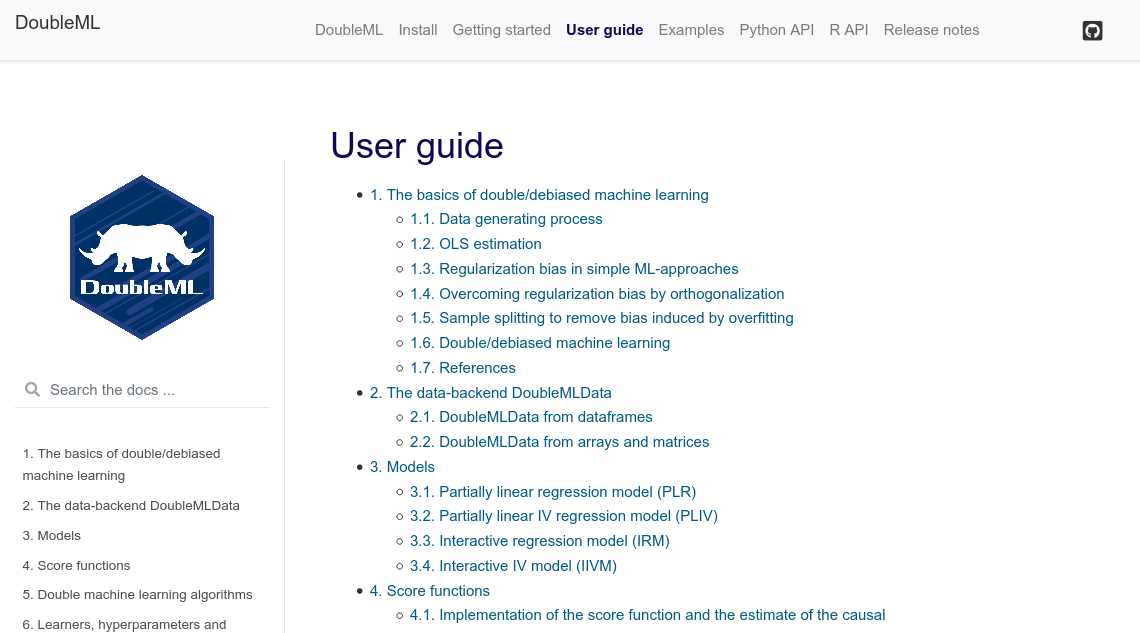
\includegraphics[width = 0.9\textwidth]{pictures_and_logos/user_guide_screenshot.png}
%\end{column}
%\begin{column}{0.5\textwidth}
%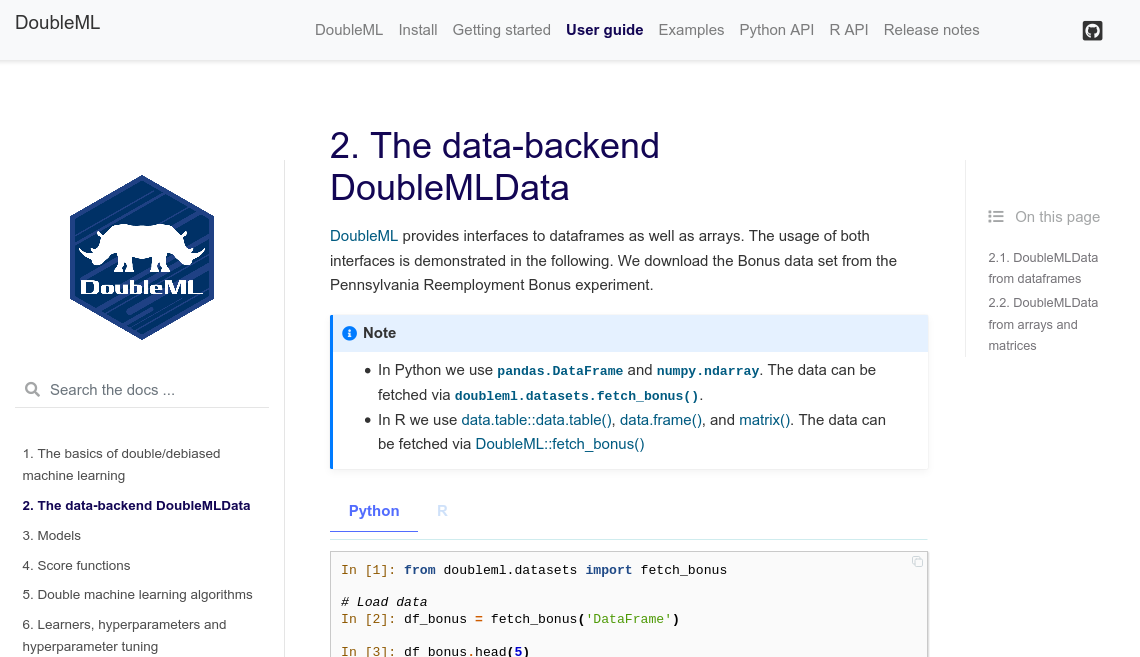
\includegraphics[width = 0.9\textwidth]{pictures_and_logos/user_guide_screenshot2.png}
%\end{column}
%\end{columns}
\end{frame}
